\documentclass[12pt,a4paper]{article}
\usepackage[utf8]{inputenc}
\usepackage[T1]{fontenc}
\usepackage[brazilian]{babel}
\usepackage[margin=2.5cm]{geometry}
\usepackage{amsmath,amssymb}
\usepackage{graphicx}
\usepackage{float}

\newcommand{\Str}{\mathit{Str}}
\newcommand{\Flw}{\mathit{Flw}}
\newcommand{\Li}{\mathit{Li}}
\newcommand{\snow}{\mathit{snow\_covered}}

\title{Inteligência Artificial -- Trabalho 2\\
\large Rede Bayesiana do Farol de Bicicleta com Dínamo}
\author{Romário Roberto de Pádua Andrade\\
Prof. Edjard Mota -- IComp/UFAM}
\date{11/10/2026}

\begin{document}
\maketitle

\section*{(a) Estrutura da Rede Bayesiana}

A topologia da rede foi estruturada modelando a causalidade física do sistema:

\begin{figure}[H]
\centering
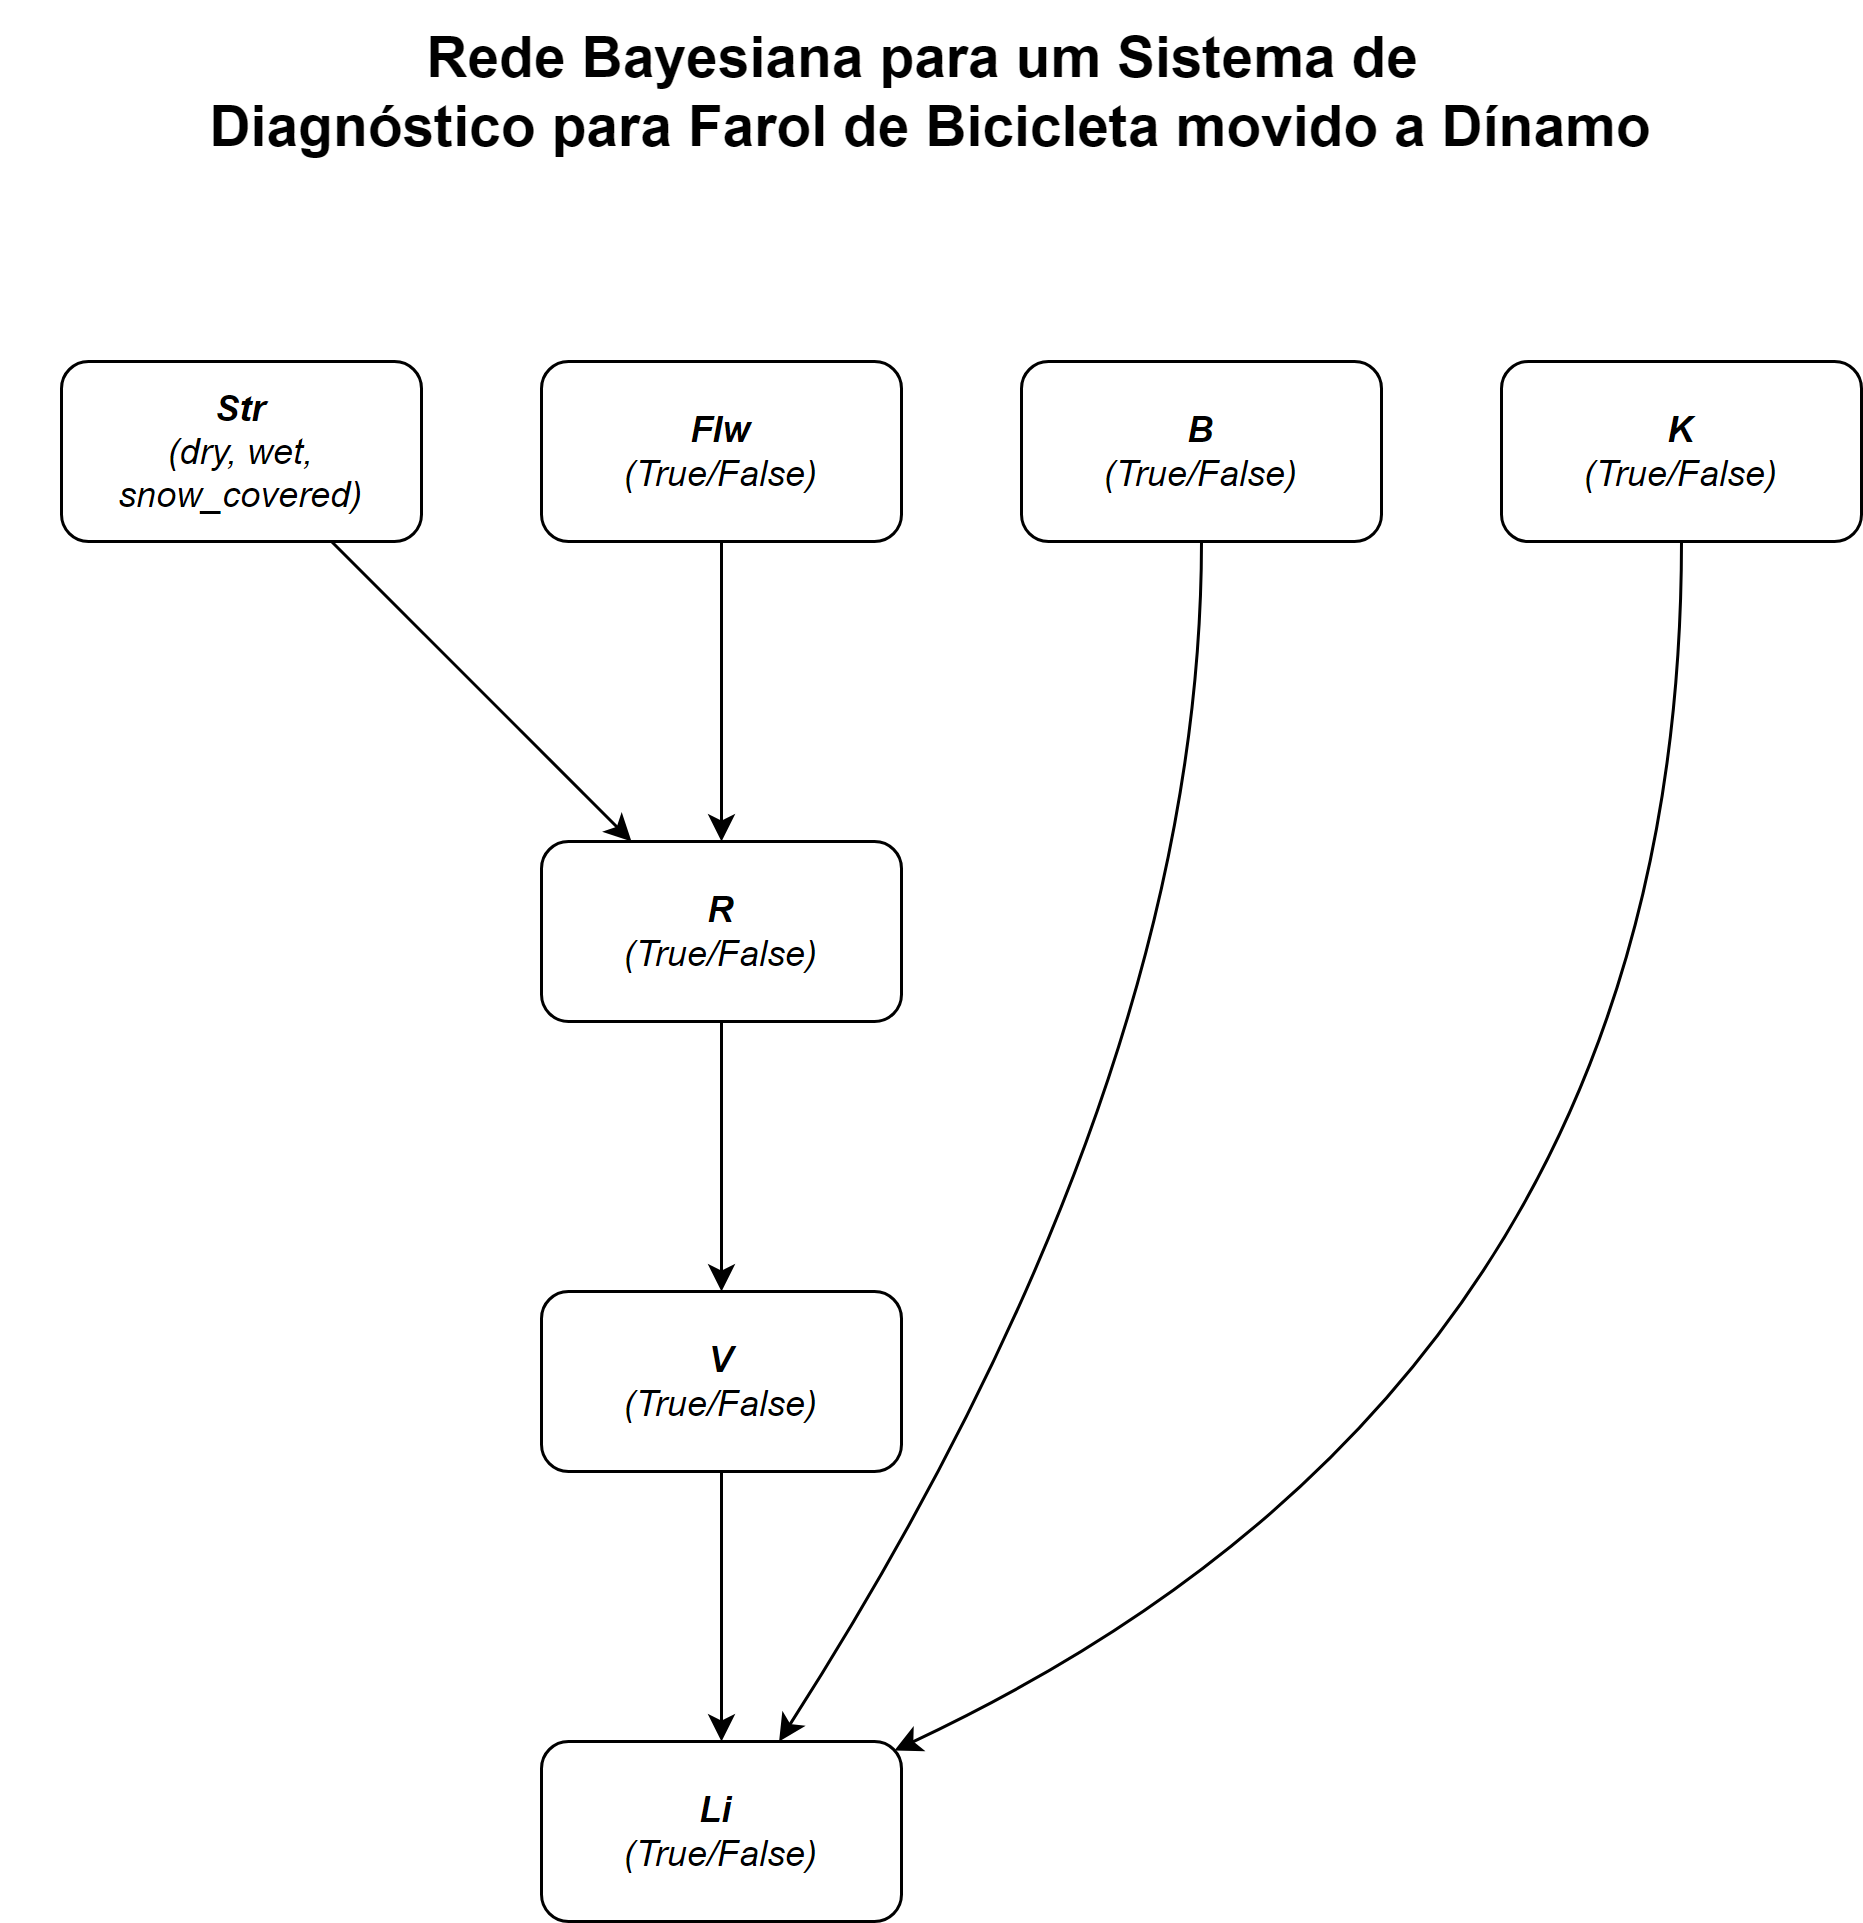
\includegraphics[width=0.75\textwidth]{bayesiana.png}
\caption{Diagrama da Rede Bayesiana para o sistema do farol de bicicleta.}
\end{figure}

A definição das arestas obedece aos seguintes critérios:
\begin{itemize}
  \item Como $\Str$, $\Flw$, $B$ e $K$ são independentes entre si, logo são os nós raiz da rede (sem ascendentes).
  \item O deslizamento do dínamo ($R$) pode ser causado pelas condições da rua ($\Str$) caso sejam adversas, ou pelo desgaste do volante ($\Flw$), justificando as arestas $\Str \to R$ e $\Flw \to R$.
  \item As relações de independência condicional $P(V \mid R, \Str) = P(V \mid R)$ e $P(V \mid R, \Flw) = P(V \mid R)$ nos mostram que a tensão gerada $V$ depende unicamente do deslizamento $R$, resultando na aresta única $R \to V$.
  \item A distribuição condicional fornecida para a lâmpada é $P(\Li \mid V, B, K)$, indicando que seus pais diretos são $V$, $B$ e $K$. A restrição $P(\Li \mid V, R) = P(\Li \mid V)$ descarta a inclusão da aresta $R \to \Li$.
\end{itemize}

\section*{(b) e (c) Especificação das Probabilidades Condicionais (CPTs)}

À exceção da distribuição de $\Li$ já fornecida, as demais CPTs foram estimadas de modo a refletir o comportamento físico esperado do sistema. Assume-se a convenção de que $P(\text{false}) = 1 - P(\text{true})$.

\paragraph{Distribuições a Priori (Nós Raiz).}

\begin{center}
\begin{tabular}{|c|c|c|c|}
\hline
$\Str$ & \textit{dry} & \textit{wet} & \textit{snow\_covered} \\
\hline
$P(\Str)$ & 0,70 & 0,20 & 0,10 \\
\hline
\end{tabular}
\end{center}

\begin{center}
\begin{tabular}{|c|c|c|}
\hline
$P(\Flw = \text{true})$ & $P(B = \text{true})$ & $P(K = \text{true})$ \\
\hline
0,10 & 0,95 & 0,97 \\
\hline
\end{tabular}
\end{center}

\paragraph{Tabela de Probabilidade Condicional para $R$.}

\begin{center}
\begin{tabular}{|c|c|c|}
\hline
$\Str$ & $\Flw$ & $P(R = \text{true} \mid \Str, \Flw)$ \\
\hline
\textit{dry}         & \text{false} & 0,01 \\
\textit{dry}         & \text{true}  & 0,20 \\
\textit{wet}         & \text{false} & 0,10 \\
\textit{wet}         & \text{true}  & 0,50 \\
\textit{snow\_covered} & \text{false} & 0,40 \\
\textit{snow\_covered} & \text{true}  & 0,90 \\
\hline
\end{tabular}
\end{center}

\paragraph{Tabela de Probabilidade Condicional para $V$.}

\begin{center}
\begin{tabular}{|c|c|}
\hline
$R$ & $P(V = \text{true} \mid R)$ \\
\hline
\text{true}  & 0,10 \\
\text{false} & 0,99 \\
\hline
\end{tabular}
\end{center}

\paragraph{Tabela de Probabilidade Condicional para $\Li$ (Fornecida).}

\begin{center}
\begin{tabular}{|c|c|c|c|}
\hline
$V$ & $B$ & $K$ & $P(\Li = \text{true} \mid V, B, K)$ \\
\hline
\text{true}  & \text{true}  & \text{true}  & 0,99  \\
\text{true}  & \text{true}  & \text{false} & 0,01  \\
\text{true}  & \text{false} & \text{true}  & 0,01  \\
\text{true}  & \text{false} & \text{false} & 0,001 \\
\text{false} & \text{true}  & \text{true}  & 0,3   \\
\text{false} & \text{true}  & \text{false} & 0,005 \\
\text{false} & \text{false} & \text{true}  & 0,005 \\
\text{false} & \text{false} & \text{false} & 0     \\
\hline
\end{tabular}
\end{center}

\section*{(d) Ausência da Aresta $(\Str, \Li)$}

A rua não age diretamente sobre a lampada ligada. Ela só influencia a lampada pelo caminho
\[
\Str \to R \to V \to \Li .
\]
Ou seja: a rua faz o dínamo deslizar ($R$), o deslizamento muda a tensão ($V$) e a
tensão decide se a luz acende. Se já sabemos $V$, saber a rua não acrescenta nada:
\[
P(\Li \mid V, \Str) = P(\Li \mid V).
\]
Por isso a aresta $\Str \to \Li$ não é necessária.

\section*{(e) Cálculo de $P(V \mid \Str = \mathit{snow\_covered})$}

Para abreviar, escreve-se $s$ para o evento $\Str = \snow$.
\renewcommand{\snow}{s}

\paragraph{Passo 1: marginalização sobre $R$.}
\[
P(V \mid \snow) = P(V \mid R, \snow)\, P(R \mid \snow)
                + P(V \mid \neg R, \snow)\, P(\neg R \mid \snow).
\]

Usando $P(V \mid R, \Str) = P(V \mid R)$:

\[
P(V \mid \snow) = P(V \mid R)\, P(R \mid \snow) + P(V \mid \neg R)\, P(\neg R \mid \snow).
\]

\paragraph{Passo 2: cálculo de $P(R \mid \snow)$, marginalizando sobre $\Flw$.}
Como $\Flw$ e $\Str$ são independentes, $P(\Flw \mid \snow) = P(\Flw)$. Assim,
\begin{align*}
P(R \mid \snow)
 &= P(R \mid \snow, \Flw)\, P(\Flw) + P(R \mid \snow, \neg \Flw)\, P(\neg \Flw) \\
 &= 0{,}90 \cdot 0{,}10 + 0{,}40 \cdot 0{,}90 \\
 &= 0{,}09 + 0{,}36 = 0{,}45 ,
\end{align*}
e, portanto, $P(\neg R \mid \snow) = 1 - 0{,}45 = 0{,}55$.

\paragraph{Passo 3: substituição.}
\begin{align*}
P(V \mid \snow) &= 0{,}10 \cdot 0{,}45 + 0{,}99 \cdot 0{,}55 \\
                &= 0{,}045 + 0{,}5445 = 0{,}5895 .
\end{align*}

\paragraph{Resposta.} $P(V = t \mid \Str = \mathit{snow\_covered}) \approx 0{,}59$. Com a rua coberta de
neve, o dínamo gera tensão em cerca de 59\% das vezes.


\end{document}